\chapter{Learning from Other Designs}
In the process of learning about nuclear engineering one undoubtedly learns a great deal about existing reactor designs. On one hand the designer should start a project with a clean slate, but on the other hand knowledge in memory can greatly accelerate the design process.
Trends, heuristics, and limitations are useful as long as the designer does not prematurely eliminate design possibilities.

In this chapter we will discuss types of nuclear reactors that have been built. The strengths and shortcomings will be listed, although not exhaustively. 
The purpose of this chapter is not to promote one design over another, because different constraints, priorities, and goals will favor different designs.

One way of classifying nuclear power reactors is by their moderator (or lack thereof) and coolant. Figure~\ref{fig:classification} is a categorization of some of the most prominent designs.

\begin{figure}[!h]
  \label{fig:classification}
  \centering
  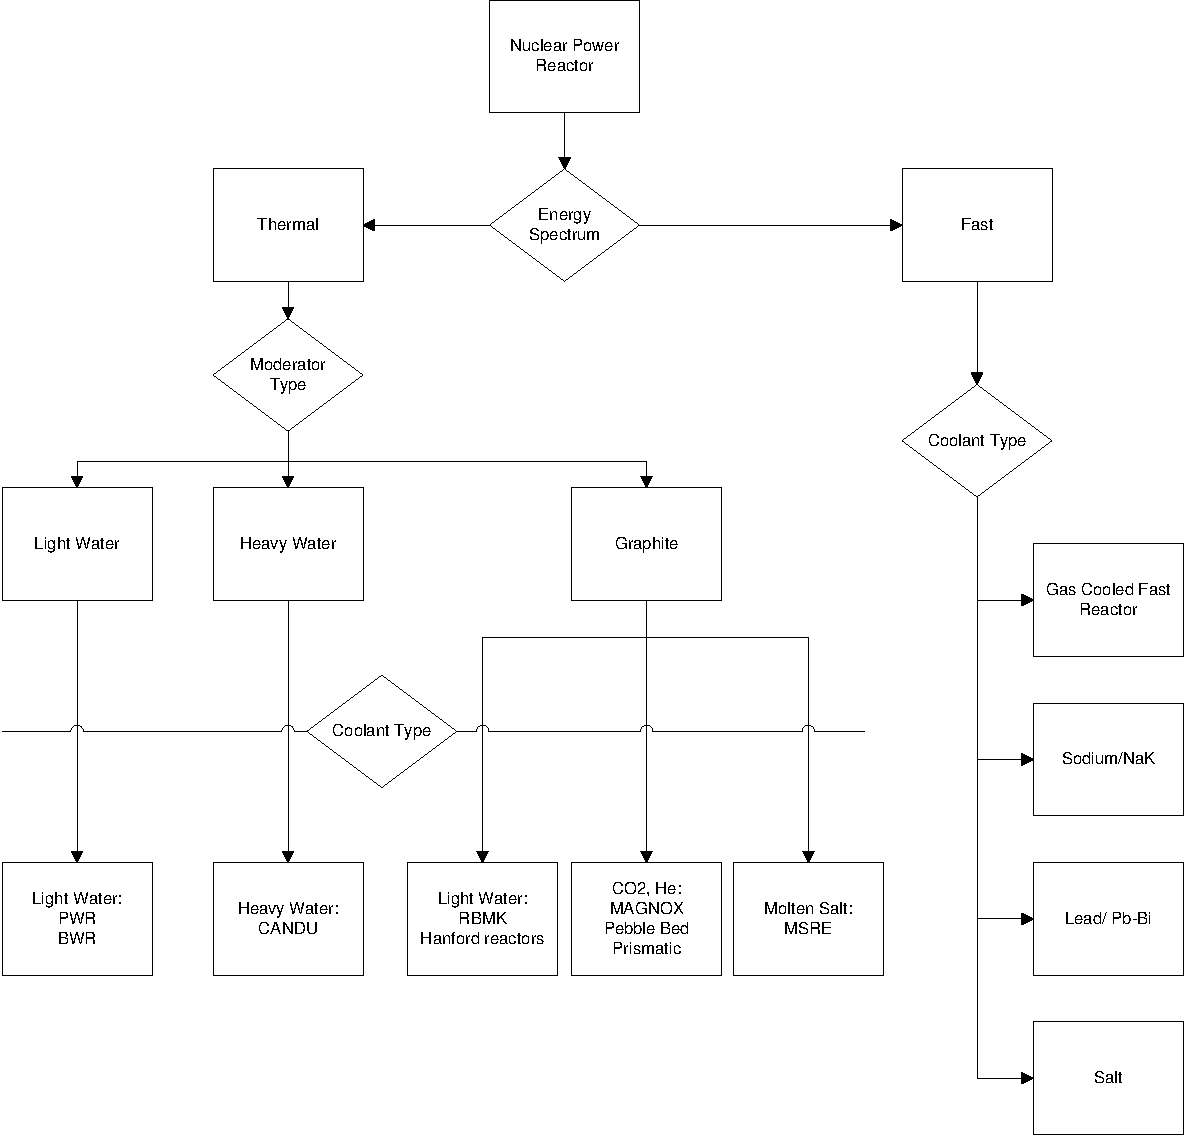
\includegraphics[width=0.90\textwidth]{graphics/RxClassification.pdf}
  \caption{One way of classifying power reactors.}
\end{figure}
\FloatBarrier

\section{Light Water Reactors}
Light water reactors are by far the most common reactor in the world. 
\begin{table}[!h]
\begin{tabular}{c|c}
  Advantages & Disadvantages \\
  \hline
  Widely used technology &  \\
  Inexpensive coolant & Corrosion issues \\
   & Requires enriched fuel \\
%  \hline
\end{tabular}
\end{table}

\subsection{Pressurized Water Reactors}
Pressurized water reactors are the more common type of light water reactor. The water must be kept high pressure to preclude boiling inside the primary coolant loop.

\subsection{Boiling Water Reactors}
Boiling Water Reactors aim for improved efficiency by using a direct power conversion cycle. However, boiling in the reactor core leads to a variety of challenges. 
\begin{table}[!h]
\begin{tabular}{c|c}
  Advantages & Disadvantages \\
  \hline
  Improved Efficiency & Two-phase flow \\
  Load following & Unstable at low power\\
   & Radioactivity in the steam turbine\\
%  \hline
\end{tabular}
\end{table}


\section{Heavy Water Reactors}
This type of reactor was developed in Canada and has since been exported around the world. The use of heavy water allows the use of un-enriched uranium. This appears to be a good feature for proliferation resistance, but the combination of on-line refueling and natural uranium leads to optimal conditions for breeding plutonium for weapons. 
The excellent neutron economy of this design may lead to extended uses in the future. For example used LWR fuel could be used as fuel in a heavy water reactor.
\begin{table}[!h]
\begin{tabular}{c|c}
  Advantages & Disadvantages \\
  \hline
  Natural uranium fuel & Expensive Moderator \\
  On-line refueling & Proliferation Risk \\
  High burnup per ore & Low burnup per fuel element \\
  No pressure vessel & Many pressure tubes \\
%  \hline
\end{tabular}
\end{table}

\section{Graphite-Moderated Water-Cooled Reactors}
These reactors are traditionally associated with weapons production. Graphite moderation allows for natural uranium fuel and efficient breeding of plutonium. The RBMK reactor in Chernobyl was not carefully designed to achieve a negative boiling reactivity coefficient, which was part of the cause of that disaster.
\begin{table}[!h]
\begin{tabular}{c|c}
  Advantages & Disadvantages \\
  \hline
  Natural uranium fuel & Large size \\
  On-line refueling & Proliferation Risk \\
  & Potential for positive reactivity coefficients \\
%  \hline
\end{tabular}
\end{table}

\section{Gas Cooled Reactors}
% One of the main benefits of using gas as a reactor coolant is that it does not change phase.  Thus the coolant is no longer a limiting factor for reactor temperature. 

\subsection{MAGNOX Reactors}

\subsection{Prismatic Block Reactors}
The fuel for these reactors is composed of millimeter-scale TRISO particles. A kernel of UO$_2$ is surrounded by several layers of graphite and silicon carbide which act as containers for fission products.
The TRISO particles are interspersed in a graphite matrix. This fuel block has various holes for coolant flow and fuel handling. Fuel blocks are stacked to compose the reactor core. 
The large mass of graphite has a very large heat capacity which can absorb the energy of almost any transient. 

Graphite reactors do have some safety issues, however. First, dislocations to the graphite atomic matrix build up with neutron fluence. The reactor must be taken to higher temperatures periodically in order to anneal the graphite and release the energy stored in these imperfections. %cite windscale
Also, there is still some debate about the flammability of graphite.
\begin{table}[!h] \label{tab:Prismatic}
\begin{tabular}{c|c}
  Advantages & Disadvantages \\
  \hline
  High heat capacity & Requires annealing\\
  High temperature ceramic & Flammable?\\
  Low absorption moderator & Large core\\
  Multiple layers around fuel & Complex manufacturing\\
  Allows high output temperature & High pumping power\\
  & Complex/large spent fuel waste\\
%  \hline
\end{tabular}
\end{table}

\subsection{Pebble Bed Reactors}
Pebble bed reactors share many features with prismatic block reactors. However, by using many fuel pebbles, better fuel economy can be achieved. %factor of two for continuous reloading, right?
Construction of the reactor core is greatly simplified: it is essentially a can with guide tubes and a bottom nozzle. 
\begin{table}[!h]
\begin{tabular}{c|c}
  Advantages & Disadvantages \\
  \hline
  Increased burnup & Complex fuel manufacturing\\
  Replaceable fuel elements & Greater likelihood of individual failure\\
   & Complex, indeterminate geometry\\
%  \hline
\end{tabular}
\caption{See Table~\ref{tab:Prismatic} for the pros and cons common to graphite reactors.}
\end{table}

\subsection{Gas-Cooled Fast Reactors}
Gas cooled fast reactors share several features with gas-cooled thermal reactors, but the lack of a large mass of graphite moderator greatly reduces the heat capacity of the reactor core. Without out this sink for energy during accidents, passive safety is much harder to attain.

The original motivation for gas cooled-fast reactors was improved neutron economy due to decreased absorption in the coolant. 
\begin{table}[!h]
\begin{tabular}{c|c}
  Advantages & Disadvantages \\
  \hline
  Single-phase coolant & High pumping power \\
  Direct cycle energy conversion & High pressure\\
   & Coolant leakage \\
  High temperature & Risk of corrosion \\
  Little absorption in coolant & Low heat capacity\\
  High breeding ratio & Low heat transfer coefficient\\
%  \hline
\end{tabular}
\end{table}


\section{Liquid Metal Cooled Reactors}
Liquid metal coolants have been considered for fast spectrum reactors since the earliest days of nuclear energy. It was the NaK-cooled Experimental Breeder Reactor (EBR-I) that first produced electricity from nuclear energy.
Liquid metals are excellent heat transfer media and also allow for the benefits of a fast-spectrum.

\subsection{Sodium(-Potassium) Cooled Fast Reactors}
Sodium is an excellent heat transfer medium, but its melting temperature is 98$^{\circ}$C. Either the coolant loops must be heated continually during shutdown, or potassium must be added to lower the melting temperature. Both metals are highly flammable. Potassium absorbs more neutrons.
\begin{table}[!h]
\begin{tabular}{c|c}
  Advantages & Disadvantages \\
  \hline
  Good heat transfer & Incompatible with air and water\\
  Fast neutron spectrum & shorter neutron lifetime\\
  Passive safety demonstrated & Sodium activated by neutrons \\
  Electronic pumping & opaque coolant\\
  & Sodium: solid at room temperature\\
  High temperature & Intermediate coolant loop\\
%  \hline
\end{tabular}
\end{table}

\subsection{Lead(-Bismuth) Fast Reactors}
Bismuth is added to lead to decrease the melting point. Lead does not react with water, air, or CO$_2$, which means intermediate cooling loops are unnecessary. 
There is less experience with lead-cooled reactors. Some Russian submarines had lead-cooled reactors, but there were eventually decommissioned.
Corrosion issues can be managed by controlling the oxygen content of the coolant. The protective oxide layer will remain intact if the coolant flow rate does not exceed about 2m/s.
\begin{table}[!h]
\begin{tabular}{c|c}
  Advantages & Disadvantages \\
  \hline
  Good heat transfer & Melting point 327$^{\circ}$C\\
  Insignificant moderation & Inelastic scattering\\
  Lead: does not absorb & Bismuth: creates Polonium\\
  Inexpensive material & very heavy\\ 
   & opaque coolant\\
  High boiling point & Erosion limit on flow rate\\
%  \hline
\end{tabular}
\end{table}


\section{Molten Salt Reactors}
Molten salt has a high heat capacity that makes it attractive as a heat transfer fluid. It can be used as a reactor coolant or as a molten fuel.
\subsection{Liquid-Fueled Reactors}
Molten salt reactors have received much attention in recent years, but have little operating experience. 
\begin{table}[!h]
\begin{tabular}{c|c}
  Advantages & Disadvantages \\
  \hline
  Good heat transfer & High Melting point \\
  High boiling point & Freezing issues\\
  Non-toxic & High activation/absorption \\
  Transparent coolant & Lacks corrosion R\&D \\
  Online reprocessing & Difficult to account for materials\\
  Little excess reactivity & Loses delayed neutrons\\
  Inherent negative expansion temperature coefficient & Loss of flow adds reactivity\\
  Non-proliferation: high gamma activity & Shielding needed throughout facility\\
%  \hline
\end{tabular}
\end{table}

\subsection{Salt-Cooled Reactors}
It may be less exotic to use molten salts as coolants rather than fuels. Thus the traditional solid fuel and cladding approach can be retained, while benefiting from the heat transfer properties of molten salts.
\begin{table}[!ht]
\begin{tabular}{c|c}
  Advantages & Disadvantages \\
  \hline
  Good heat transfer & High Melting point \\
  High boiling point & Freezing issues\\
  Non-toxic & High activation/absorption \\
  & Highly positive coolant temperature coefficient\\
  Transparent coolant & Lacks corrosion R\&D \\
  High heat capacity & Low thermal conductivity \\ 
%  \hline
\end{tabular}
\end{table}

\section{Homework Problems}
\begin{enumerate}
\item Research a reactor that you don't know much about and list its advantages and disadvantages. (Interesting reactors include: organic-cooled reactors, research reactors such as TRIGA, aircraft propulsion reactors, space reactors, salt-cooled pebble-bed reactors, etc.)
\item Choose two reactors types from this chapter and compare their strengths and weaknesses. What applications is each one best suited for? Which set of strengths and weaknesses would you prefer for a) minimizing the levelized cost of power and b) minimizing the generation of nuclear waste?
\end{enumerate}
